\documentclass[a4paper,10pt,twoside]{article}
%\usepackage{amssymb}
%\usepackage{amsthm}
\usepackage[polish]{babel}
\usepackage[utf8]{inputenc}
\usepackage[T1]{fontenc}
\usepackage{indentfirst}
\usepackage[top=2.5cm, bottom=2.5cm, left=2.5cm, right=2.5cm]{geometry}
\usepackage{booktabs}
\usepackage{graphicx}
\usepackage{float}
\usepackage{wrapfig}
%\usepackage{xcolor}
\usepackage{amsmath}

\begin{document}

\newgeometry{top=1.5cm,bottom=2.5cm,left=2.5cm,right=2.5cm}
\begin{center}
\bgroup
\def\arraystretch{1.5}
\begin{tabular}{|c|c|c|c|c|c|}
	\hline
	EAIiIB & \multicolumn{2}{|c|}{\begin{tabular}{@{}c@{}}Marcin Nalepa \\ Przemysław Trybała\end{tabular}} & Rok II & Grupa 5 & Zespół 3 \\
	\hline
	\multicolumn{3}{|c|}{\begin{tabular}{c}Temat: \\ Wahadło fizyczne \end{tabular}} & 
	\multicolumn{3}{|c|}{\begin{tabular}{c}Numer ćwiczenia: \\ 1 \end{tabular}} \\
	\hline
	\begin{tabular}{@{}c@{}}Data wykonania\\09.12.2015 r.\end{tabular} & \begin{tabular}{@{}c@{}}Data oddania\\13.01.2016 r.\end{tabular} & 
	\begin{tabular}{c}Zwrot do\\poprawki\\\phantom{data} \end{tabular} & \begin{tabular}{c}Data oddania\\\phantom{data}\end{tabular} &
	\begin{tabular}{c}Data zaliczenia\\\phantom{data}\end{tabular} & \begin{tabular}{c}Ocena\\\phantom{ocena}\end{tabular} \\[4ex]
	\hline
\end{tabular}
\egroup
\end{center}

\section{Cel ćwiczenia}
Wyznaczenie momentów bezwładności brył sztywnych przez pomiar okresu drgań wahadła oraz na podstawie wymiarów geometrycznych.

\section{Wstęp teoretyczny}
\emph{Wahadłem fizycznym} nazywamy bryłę sztywną mogącą obracać się swobodnie wokół osi obrotu $O$
nie przechodzącej jednak przez środek masy $S$ tej bryły.

\begin{wrapfigure}{r}{0.4\textwidth}
	%\vspace{-30pt}
	\begin{center}
		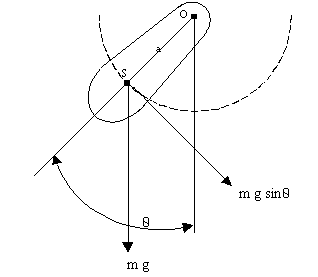
\includegraphics[scale=0.7]{wahadlo}
	\end{center}
	%\vspace{-20pt}
	\caption{Rysunek poglądowy doświadczenia}
	\label{fig:wahadlo}
\end{wrapfigure}

Wahadło wychylone z punktu równowagi, a następnie puszczone swobodnie, będzie wykonywać drgania zwane ruchem wahadłowym.
Ponieważ ciało będzie poruszać się wokół osi obrotu $O$, ruch ten będzie opisywać druga zasada dynamiki dla ruchu obrotowego
$I\varepsilon=\mathbf{M}$ gdzie $I$ - moment bezwładności, $\varepsilon$ - przyspieszenie kątowe, $\mathbf{M}$ - moment siły.

W rozpatrywanym doświadczeniu moment siły powstaje pod wpływem siły ciężkości i dla wychylenia $\theta$ jest równy $\mathbf{M} = mga\sin\theta$,
gdzie $a$ - odległość osi obrotu $O$ od środka masy $S$. Stąd równanie ruchu wahadła można zapisać jako
\begin{equation}
\label{eq:wahadlo}
I_0\frac{d^2\theta}{dt^2}=-mga\sin\theta
\end{equation}
gdzie $I_0$ - moment bezwładności względem osi obrotu przechodzącej przez punkt $O$. Jeśli ograniczymy amplitudę drgań wahadła do kilku stopni,
możemy, zgodzie z twierdzeniem Taylora, przyliżyć sinusa jego argumentem $\sin\theta\approx\theta$. Wtedy rozwiązanie wzoru (\ref{eq:wahadlo})
przyjmuje postać
\begin{equation}
\label{eq:oscylator}
\theta = A \cos\left(\omega_0t+\alpha\right)
\end{equation}
i przedstawia ruch harmoniczny. Amplituda $A$ oraz faza drgań $\alpha$ zależą od warunków początkowych, natomiast okres drgań $T$ jest związany tylko
z częstością $\omega_0=2\pi/T$ i wynosi
\begin{equation}
T = 2\pi\sqrt{\frac{I_0}{mga}}
\end{equation}
co po przekształceniu daje wzór roboczy na moment bezwładności $I_0$
\begin{equation}
\label{eq:bezwladnosc}
I_0 = \frac{T^2mga}{4\pi^2}
\end{equation}

Wzór (\ref{eq:bezwladnosc}) jest pierwszą metodą na obliczenie momentu bezwładności wahadła fizycznego. Drugi sposób to zastosowanie
twierdzenia Steinera
\begin{equation}
\label{eq:steiner}
I_0 = I_s + ma^2
\end{equation}
do znanej wartości $I_s$ odczytanej z tablic.

\section{Opis doświadczenia}
Do doświadczenia zostały dostarczone 2 obiekty, pierścień i pręt. Na początku zostały przeprowadzone pomiary potrzebnych wymiarów
zaznaczonych na rysunku (\ref{fig:prety}) oraz masy. Wyniki wraz z niepewnościami zapisano w dołączonych tablekach. 
\begin{figure}[H]
\centerline{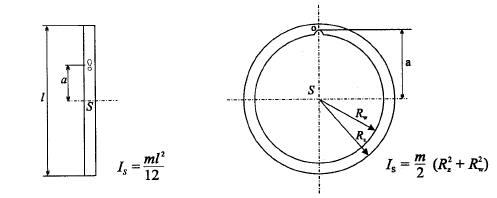
\includegraphics[scale=0.5]{prety}}
\label{fig:prety}
\end{figure}

Następnie jeden z obiektów zamontowano na statywie i zmierzono czas trwania określonej ilości okresów. Stąd wyznaczono okres 1 drgania.
Pomiary zostały wykonane także dla drugiego obiektu. Wyniki zapisano w dołączonych tabelach.

\newpage
\section{Opracowanie wyników}
\noindent
Wzory wykorzystane w obliczeniach poniżej:
\begin{itemize}
\item Moment bezwładności: $I_0=\frac{mgaT^2}{4\pi ^2}$
\item Niepewność $I_0$: $\frac{u(I_o)}{I_0}=\sqrt{\left (\frac{u(m)}{m}\right ) ^2+\left ( \frac{u(a)}{a}\right )^2+\left (2 \frac{u(T_0)}{T_0}\right )^2}$
\item Moment bezwładności z twierdzenia Steinera (\ref{eq:steiner}): $I_s=I_0-ma^2$
\item Niepewność $I_S$: $u(I_s)=\sqrt{\left( u(I_0)\right)^2+\left(a^2u(m) \right)^2+\left( -2amu(m)\right)^2}$
\end{itemize}

\subsection{Pręt}
\subsubsection{Pomiar długości drgań i twierdzenie Steinera}
$$I_0=\frac{0,66*9,81*0,27*1,33^2}{4\pi ^2}=0,07838~[kg*m^2]$$
Niepewność $u(I_0)$:
\begin{equation*}
\begin{split}
\frac{u(I_o)}{I_0}&=\sqrt{\left(\frac{0,00058}{0,657}\right) ^2+\left( \frac{0,00058}{0,271}\right)^2+\left(2 \frac{0,0018}{1,325}\right)^2}\\
&= \sqrt{7,8*10^{-7}+4,58*10^{-6}+7,4*10-6} = \sqrt{12,76*10^{-6}} = 0,00357
\end{split}
\end{equation*}
Stąd $u(I_0)=0,00028~[kg*m^2]$
\newline

\noindent
Z twierdzenia Steinera (\ref{eq:steiner}) mamy dla środka ciała:
$$I_s=0,07838-0,657*0,27^2=0,0305~[kg*m^2]$$
a niepewność $I_s$ liczymy ze wzoru:
$$u(I_s)=\sqrt{\left( 0,00028\right)^2+\left(0,27^2*0,00058 \right)^2+\left( -2*0,27*0,66*0,00058\right)^2}=0,00035~[kg*m^2]$$
\subsubsection{Wzory tablicowe}
$$I_{s}^{geom}=\frac{ml^2}{12}=\frac{0,657*0,74^2}{12}=0,0298~[kg*m^2]$$
Niepewność $u(I_{s}^{geom})$:
\begin{equation*}
\begin{split}
u(I_{s}^{geom})&=\sqrt{\left(\frac{l^2}{12}*u(m) \right)^2+\left(\frac{2lm}{12}*u(l) \right)^2}\\
&=\sqrt{\left (\frac{0,74^2}{12}*0,00058 \right )^2+\left (\frac{2*0,74*0,657}{12}*0,00058 \right )^2}=0,000054~[kg*m^2]
\end{split}
\end{equation*}


\newpage
\subsection{Pierścień}
\subsubsection{Pomiar długości drgań i twierdzenie Steinera}
$$I_0=\frac{1,36*9.81*0,13*1,033^2}{4\pi ^2}=0,04693~[kg*m^2]$$
Niepewność $u(I_0)$:
\begin{equation*}
\begin{split}
\frac{u(I_o)}{I_0}&=\sqrt{\left(\frac{0.00058}{1,36}\right) ^2+\left( \frac{0.00058}{0,13}\right)^2+\left(2 \frac{0.0016}{1,033}\right)^2}\\
&= \sqrt{1,819*10^{-7}+1,99*10^{-5}+9,6*10^{-6}} = \sqrt{2,97*10^{-5}} = 0,00545
\end{split}
\end{equation*}
Stąd $u(I_0)=0,00026~[kg*m^2]$
\newline

\noindent
Z twierdzenia Steinera (\ref{eq:steiner}) mamy dla środka ciała:
$$I_s=0,04693-1,36*0,13^2=0,0239~[kg*m^2]$$
a niepewność $I_s$ liczymy ze wzoru:
$$u(I_s)=\sqrt{\left( 0,00026\right)^2+\left(0,13^2*0,00058 \right)^2+\left( -2*0,13*1,36*0,00058\right)^2}=0,00033~[kg*m^2]$$
\subsubsection{Wzory tablicowe}
$$I_{s}^{geom}=\frac{m(R_z^2+R_w^2)}{2}=\frac{1,36(0,14^2+0,125^2)}{2}=0,024~[kg*m^2]$$
Niepewność $u(I_{s}^{geom})$:
\begin{equation*}
\begin{split}
u(I_{s}^{geom})&=\sqrt{\left (\frac{R_z^2+R_w^2}{2}*u(m) \right )^2+\left (mR_z*u(R_z) \right )^2+\left (mR_w*u(R_w) \right )^2}\\
&=\sqrt{\left (\frac{0,14^2+0,125^2}{2}*0,00058 \right )^2+\left (1,36*0,14*0,00058 \right )^2+\left (1,36*0,125*0,00058 \right )^2}\\
&=\sqrt{10^{-10}+1,2*10^{-8}+9,7*10^{-9}}=0,000148~[kg*m^2]
\end{split}
\end{equation*}


\newpage
\subsection{Sprawdzenie wyników}
\noindent
\begin{itemize}
\item $k=2$
\item $U\left(I_s-I_{geom} \right)=k*\sqrt{u(I_s)^2+u(I_{geom})^2)}$
\item sprawdzenie: $\left | I_s - I_{geom} \right | < U(I_s-I_{geom})$
\end{itemize}

\subsubsection{Pręt}
\begin{table}[H]
\centering
\def\arraystretch{1.4}
\begin{tabular}{|c|c|c|}
	\hline
	& $I_s$ z pomiarów & $I_s^{geom}$ tablicowe \\
	\hline
	wartość $[kg*m^2]$ & 0,0305 & 0,02980 \\
	\hline
	niepewność $[kg*m^2]$ & 0,0004 & 0,00005 \\
	\hline
\end{tabular}
\end{table}
\begin{align*}
U\left(I_s-I_s^{geom} \right)&=0,0008~[kg*m^2]\\
\left| I_s-I_s^{geom} \right|&=0,0305-0,0298=0,0007~[kg*m^2]
\end{align*}
zgodne ponieważ $0,0007 < 0,0008$

\subsubsection{Pierścień}
\begin{table}[H]
\centering
\def\arraystretch{1.4}
\begin{tabular}{|c|c|c|}
	\hline
	& $I_s$ z pomiarów & $I_s^{geom}$ tablicowe \\
	\hline
	wartość $[kg*m^2]$ & 0,0239 & 0,0240 \\
	\hline
	niepewność $[kg*m^2]$ & 0,0003 & 0,0001 \\
	\hline
\end{tabular}
\end{table}
\begin{align*}
U\left(I_s-I_s^{geom} \right)&=0,0006~[kg*m^2]\\
\left| I_s-I_s^{geom} \right|&=0,024-0,0239=0,0001~[kg*m^2]
\end{align*}
zgodne ponieważ $0,0001 < 0,0006$


\section{Podsumowanie}
Momenty bezwładności obliczone z pomiaru czasu drgań wahadła wynoszą odpowiednio $0,0305 \pm 0,0004~[kg*m^2]$ dla pręta i $0,0239 \pm 0,0003~[kg*m^2]$ dla pierścienia.
Wartości momentu bezwładności mieszczą się w niepewności rozszerzonej. Oznacza to, że pomiary były wykonane na tyle dokładnie, że wyniki
zgadzają się z wartościami oczekiwanymi. W obu przypadkach niepewności liczone ze wzorów matematycznych charakteryzują się większą dokładnością, a więc
są pewniejsze niż wartości doświadczalne. Taki stan rzeczy może być spowodowany tym, że w przypadku pomiaru okresu drgań pojawia się błąd systematyczny
związany z tłumieniem drgań przez powietrze. 

\end{document}


























